% made this in the slides for week 8 lol

\question Munchlax is hungry (no surprise there) and wants your help to find her way to the tasty poffins. The problem is, she doesn't know which doors lead to poffins and which don't. Suggest a method of finding which doors have poffins behind them and which don't. 

%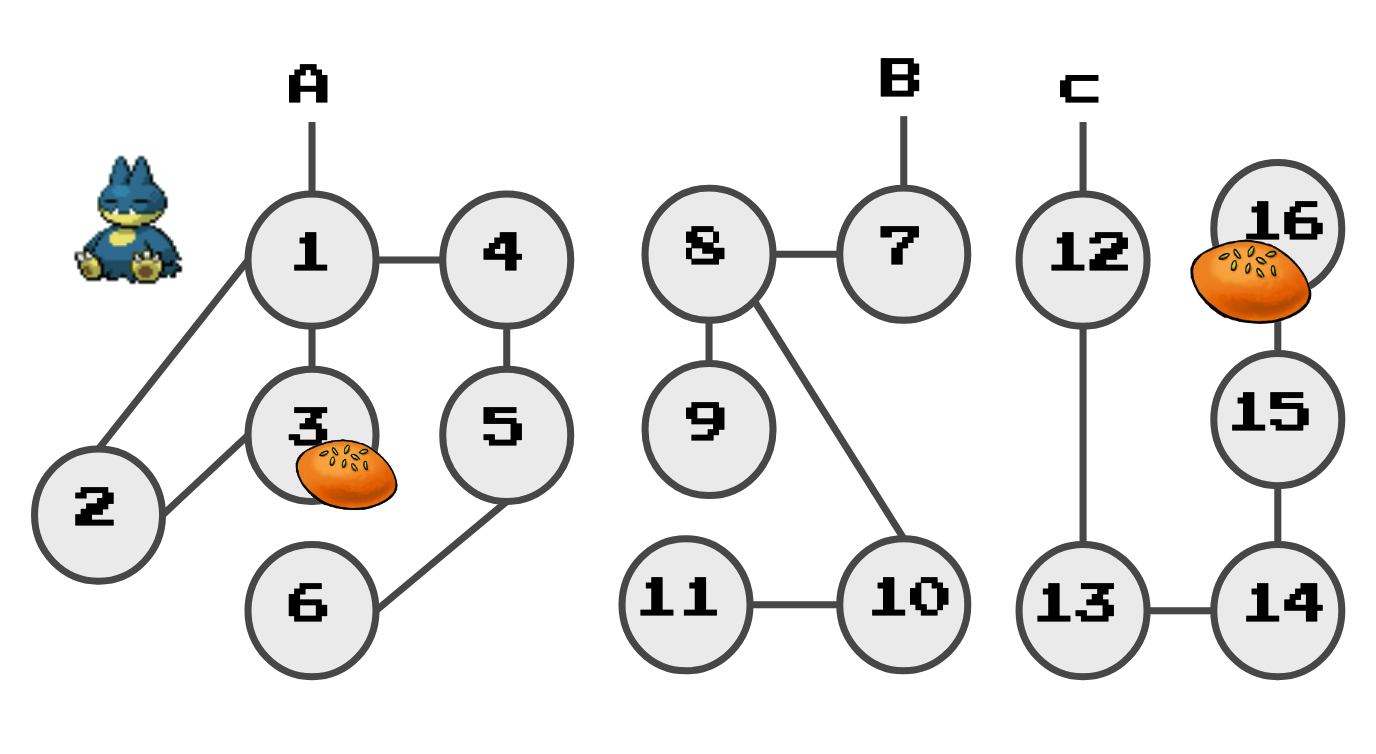
\includegraphics[width=\marginparwidth, scale = 2]{topics/graphs/images/munch-graph.png}
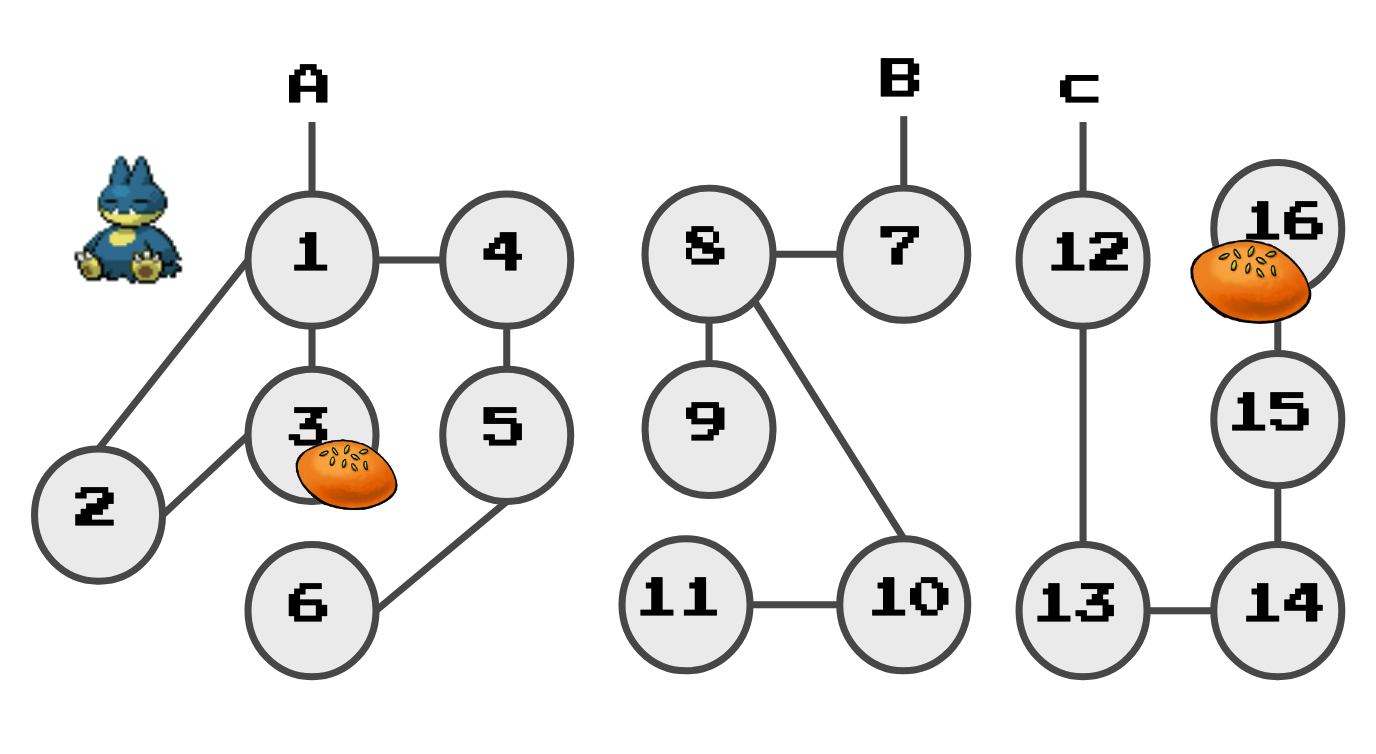
\includegraphics[scale = 0.5]{topics/graphs/images/munch-graph.png}

\begin{solution}
We could use a local DFS on a particular node, or BFS. BFS takes in a root as an argument while DFS doesn't, so BFS will always work but DFS will only work if modified to work from a particular root. Answers that only list DFS with no modifications are incorrect.  
\end{solution}
\vspace{45mm}

% \question Munchlax is glad to know where the poffins are located, but is awful lazy and will give up if she has to go too far to get her poffins. She also doesn't like thinking very hard. To solve both issues, provide an asymptotically fast method of finding only poffins less than 3 steps away from Munchlax's current location (we define the first node beyond a door as the 1st step. 1, 7, and 12 are the 1st steps of $A$, $B$, and $C$ respectively.) Additionally, provide a runtime for this method in terms of $V$ (vertex count) and $E$ (edge count). No proof necessary, only the explanation of your approach.

% \begin{solution}
% Modify BFS to stop after getting to the 4th level. This requires an implementation of BFS which keeps track of level - which while not standard is not difficult to do. This would take $O(V + E)$ time.\\

% Modifying DFS to do something similar would take much more time and thus would be incorrect. 
% \end{solution}
% \vspace{45mm}

\question Give the pre and post ordering of the graph starting from door $A$ (the door itself is not a node). Suppose we break ties in numerical order. 

\begin{solution}
Pre-ordering: 1, 2, 3, 4, 5, 6

Post-ordering: 3, 2, 6, 5, 4, 1
\end{solution}

\vspace{30mm}

\question (Challenge, Optional) Ekans, a good friend of Munchlax wants to take a walk through the entire graph of all three disjoint parts following only one DFS traversal starting from door $A$ such that the pre-ordering is the reverse of the post-ordering. Give the shortest possible list of added edges we would need to make this possible. Suppose we break ties in numerical order. 

\begin{solution}
We just connect any neighboring numbers that aren't already connected by an edge directly between them. 
(3,4), (6,7), (9, 10), (11,12)
\end{solution}